\documentclass{article}
\usepackage[margin=1in]{geometry}
\usepackage{amsmath,amsthm,amssymb}
\usepackage{bbm,enumerate,mathtools}
\usepackage{tikz,pgfplots}
\usepackage{chessboard}
\usepackage[hidelinks]{hyperref}
\usepackage{multicol} % Problem 35

\newenvironment{question}{\begin{trivlist}\item[\textbf{Question.}]}{\end{trivlist}}
\newenvironment{note}{\begin{trivlist}\item[\textbf{Note.}]}{\end{trivlist}}
\newenvironment{references}{\begin{trivlist}\item[\textbf{References.}]}{\end{trivlist}}
\newenvironment{related}{\begin{trivlist}\item[\textbf{Related.}]\end{trivlist}\begin{enumerate}}{\end{enumerate}}


\begin{document}
\rating{3}{2}
For each $2n$-gon there exists some number $\ell_n$ such that there is a
equilateral convex polygon with integer coordinates such that all sides have
length $\ell_n$.
\begin{figure}[ht!]
  \centering
  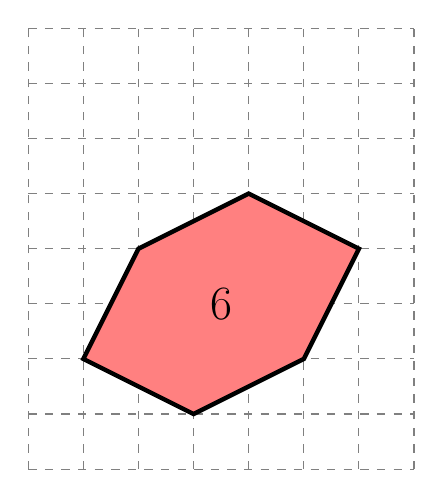
\begin{tikzpicture}[scale=0.7]
    \draw[gray, dashed] (0,0) grid (7,8);
    \draw[ultra thick, fill=red!50] (1,2)--(2,4)--(4,5)--(6,4)--(5,2)--(3,1)--cycle;
    \node at (3.5,3) {\LARGE 6};
  \end{tikzpicture}\hspace{1cm}
  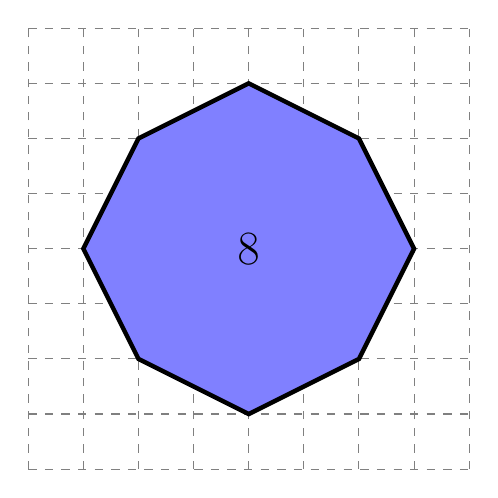
\begin{tikzpicture}[scale=0.7]
    \draw[gray, dashed] (0,0) grid (8,8);
    \draw[ultra thick, fill=blue!50] (2,2)--(1,4)--(2,6)--(4,7)--(6,6)--(7,4)--(6,2)--(4,1)--cycle;
    \node at (4,4) {\LARGE 8};
  \end{tikzpicture}
  \caption{
    Example demonstrating that $\ell_6 = \ell_8 = \sqrt{5}$.
  }
\end{figure}
\begin{question}
  For what values of $m$ do there exist equilateral $(2m-1)$-gons with integer
  coordinates?
\end{question}

\begin{related}
  \item For $m$ such that there are no equilateral $(2m-1)$-gons, what is do
    the best Diophantine approximations look like (in the sense of
    Problem 62)?
  \item Does this generalize to polyhedra?
\end{related}
\begin{references}
  \item \url{https://oeis.org/A071383}
  \item Problem 62
\end{references}
\end{document}
